\begin{frame}{Single Slab}
    Given a hyperplane $P = \left\{\mathbf x \mid \mathbf n^\intercal \mathbf x = b\right\} \subset \mathbb R^n$.
    \textbf{A $\delta$–slab} defined by hyperplane $P$, is given by:
    \[
    Slab_\delta(P) \stackrel{\text{def}}{=} \left\{\mathbf x \in \mathbb R^n \mid d(\mathbf x, P) < \delta \right\} \subset \mathbb R^n, \quad \text{for } \delta \in \mathbb R
    \]

    \begin{figure}[H]
        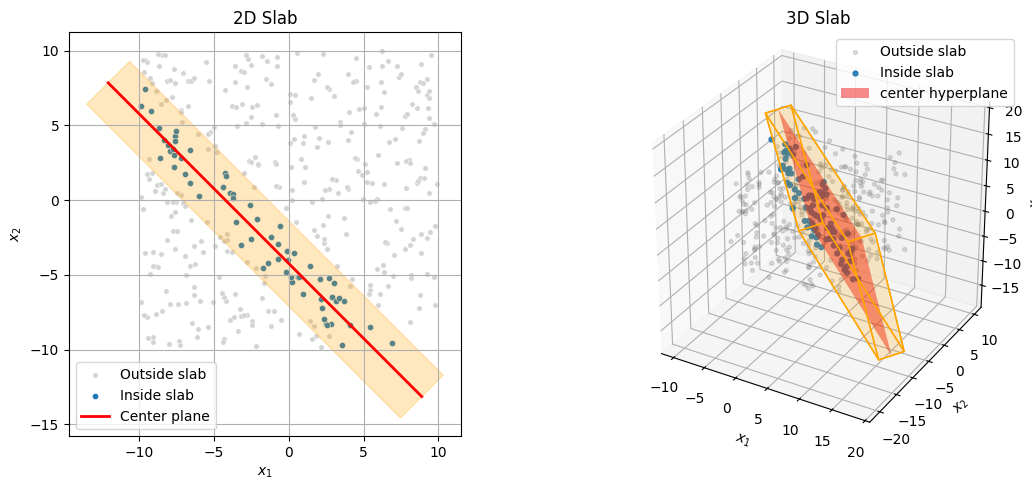
\includegraphics[width=0.95\textwidth]{figures/fig_11.png}
        \label{fig:fig_11}
    \end{figure}
\end{frame}